\section{State-of-the-Art}
\label{sec:sota}

Bereits seit den 1950er Jahren wurden strömungsdynamische Ansätze für die Simulation von Verkehrsflüssen entwickelt. 
Außerdem gab es ab den 1980er Jahren auch boolsche Simulationsmodelle, die mit Gitter-Gas-Automaten Flüssigkeiten simulieren konnten.
Anfang der 1990er wurde von Kai Nagel und Michael Schreckenberg in \cite{na-sch} ein Verfahren vorgestellt, welches Autobahnverkehr basierend auf Zellularautomaten modelliert. 

\begin{quote}
Ein zellulärer Automat ist eine regelmäßige Annordnung von Zellen. Jede Zelle kann eine endliche Zahl von Werten / Zuständen annehmen und hat eine  begrenzte Zahl von Nachbarzellen, die sie beeinflussen können. Das Muster des gesamten zellulären Automaten ändert sich in einzelnen Schritten, die durch eine Reihe von Übergangsregeln bestimmt werden, die für alle Zellen gelten.\footnote{aus \cite{cell-autom}}
\end{quote}

Vereinfacht kann eine Fahrspur einer Straße als Aneinanderreihung vieler solcher Zellen gesehen werden. 
Dies führt schließlich zu einer gridbasierten Simulationsumgebung. 
In \cite{na-sch} wird die Rechenumgebung als eindimensionales Array mit $L$ Zellen definiert. 
Jede der Zellen kann entweder von einem Fahrzeug belegt oder frei sein. 
Eine Simulation in dieser Grid-Welt hat den Vorteil, dass die Erkenntnisse auf die reale Welt skaliert werden können. 
Es wird von einer Zelllänge von 7,5 m\footnote{\cite{na-sch}, S. 2227} ausgegangen, was ungefähr dem beanspruchten Platz eines Pkw - Fahrzeugfront zu Fahrzeugfront - in einer Stausituation entspricht (Fahrzeuglänge + Abstand). 
Jedes Fahrzeug hat eine ganzzahlige Geschwindigkeit zwischen null und $v_{max}$.

\begin{table}[ht]
\begin{center}
\setlength{\tabcolsep}{0.5em} % for the horizontal padding
{\renewcommand{\arraystretch}{1.2}% for the vertical padding
\begin{tabular}{| c | c | c |}
\hline 
$v^{sim}$ in $\frac{Zellen}{Zeitschritt}$ & $\widehat{=}$ $v^{real}$ in $\frac{m}{s}$ & $\frac{km}{h}$ \\ \hline 
$1$ & 7,5 & 27 \\ \hline
$2$ & 15 & 54 \\ \hline
$3$ & 22,5 & 81 \\ \hline
$4$ & 30 & 108 \\ \hline
$5$ & 37,5 & 135 \\ \hline
$6$ & 45 & 162 \\ \hline
\end{tabular}
}
\end{center}
\caption{Umrechnung Geschwindigkeiten Gridwelt $\rightarrow$ reale Welt}
\label{tab:umrechnung-zelle-kmh}
\end{table}

Die beobachtete Durchschittsgeschwindigkeit von 4,5 Zellen/Zeitschritt, der als eine Sekunde angenommen wird, entspricht etwa der einer Geschwindigkeit von 120 km/h\footnote{\cite{na-sch}, S. 2227}. 

In \cite{na-sch} war es erstmals gelungen, Wechselwirkungen zwischen Fahrzeugen im Einspurfall darzustellen \sa{...auf der Basis einen theoretischen Modells zu entwickeln... $\Rightarrow$ mit 1-2 Sätzen die Kernaussagen der Arbeit von Dat beschreiben} und u.a. das Entstehen von Staus zu modellieren. 
Mit drei Regeln, die auf jedes Fahrzeug gleichzeitig und gleichermaßen anzuwenden waren, wurde ein realistischer Verkehrsfluss generiert. 
Die folgenden Regeln, die die Kollisionsfreiheit sichern, sind die Grundlage für die heute als "Nagel-Schreckenberg-Modell" bekannte Modellierung:\pk{Hier ist kein Schritt von Dat zu NaSch} 

\begin{itemize}
\item Beschleunigung: Solange ein Fahrzeug nicht seine max. Geschwindigkeit $v$ (Zellen/Zeitschritt) erreicht hat und ein vorausfahrendes Fahrzeug weit genug entfernt ist, dann erhöhe die Geschwindigkeit um $1$, $v \rightarrow v+1$;
\item Abbremsen: Hat ein Fahrzeug ein anderes Fahrzeug $j$ Schritte vor sich, dann reduziert es die Geschwindigkeit auf $j-1$, $v \rightarrow j-1$;
\item Zufallsgröße, auch 'Trödelwahrscheinlichkeit': Mit einer Wahrscheinlichkeit $p$ wird die Geschwindigkeit ($v > 0$) eines Fahrzeuges um $1$ reduziert, $v \rightarrow v-1$
\end{itemize}

Die Anweisungen werden, gleichzeitig für alle Fahrzeuge, in der angegebenen Reihenfolge ausgeführt und jedes Fahrzeug um die entsprechende Anzahl Zellen weiter gesetzt.

Dehnte man dieses Modell aber auf mehrere Fahrspuren aus, stößt es an seine Grenzen, weil die Modellierung von Überholvorgängen, genannt "Ausscheren" und "Einscheren", nicht Teil des ursprünglichen Modells ist. \cite{multi-lane} liefert eine 'multi-lane'-Betrachtung, wobei die ursprünglichen Regeln durch weitere ergänzt 
.\sa{bist Du Dir mit \textit{ergänzt} wirklich sicher?} 
.\pk{\textit{ergänzt} vs. \textit{erweitert}} werden, die zum einen das Auffahren auf den die Spur wechselnden und des die Spur wechselnden nach dem Spurwechsel verhindern. \\
In der Betrachtung, ob die Aktualisierung der Fahrzeuge parallel oder sequentiell erfolgen soll, wurde erkannt, dass dies für das entwickelte Modell nur geringe Unterschiede macht, da die Rate der Spurwechsel mit den festgelegten Regeln eher gering ist. \\
Gleichzeitung wurde auch beobachtet, dass Fahrzeuge nicht wieder von der Überholspur in die Normalspur wechselten. Dies wurde mit weiteren Regeln und einer Spurwechselwahrscheinlichkeit abgestellt. Eine weitere Kalibrierung des Modells wurde in einer Folgearbeit durchgeführt. \\
Durch die Konstanthaltung der Anzahl generierter Fahrzeuge und die Veränderung der Systemgröße konnten verschiedene Verkehrsdichten simuliert werden.\sa{evtl diese Punkte von \glqq In der Betrachtung\grqq\ als Itemlist und dann den Text kürzen} 

\cite{multi-lane} zeigt mehrere Diagramme. Eine Untersuchung der realen Spurwechselvorgänge ergab, dass eine Umkehr der Benutzungshäufigkeit der rechten und linken Spuren bei einem Verkehrsfluss $q_{12}$ von etwa 1200 (Fahrzeugen) pro Stunde auf beiden Spuren.

Die Simulation ergab, dass der Punkt, an dem beide Spuren gleichermaßen benutzt werden, deutlich unter dem Punkt liegt, an dem der maximale Verkehrsfluss erreicht wird, siehe \cref{figure:verkehrsfluss-spurnutzung}.

\begin{figure}[hptb]
 \centering
 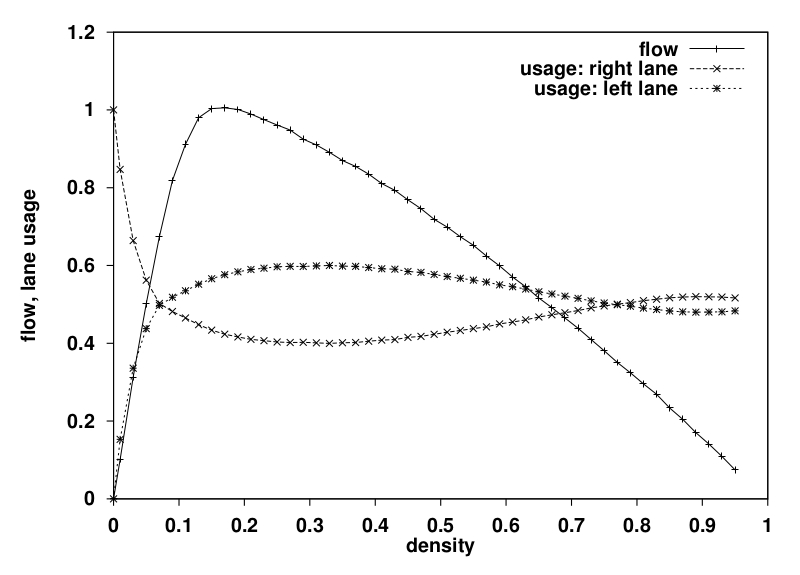
\includegraphics[width=0.75\textwidth]{verkehrsfluss-spurnutzung}
 \caption[Verkehrsfluss und Spurnutzung als Funktion der Verkehrsdichte]{Verkehrsfluss und Spurnutzung als Funktion der Verkehrsdichte, aus \cite{multi-lane}}
 \label{figure:verkehrsfluss-spurnutzung}
\end{figure}

Ein weiteres Resultat der Simulation ist eine mehrfache Umkehr der Nutzung der Fahrspuren abhängig von der Verkehrsdichte, wenn andere Parameter konstant gehalten werden, siehe \cref{figure:verkehrsfluss}.

\begin{figure}[hptb]
 \centering
 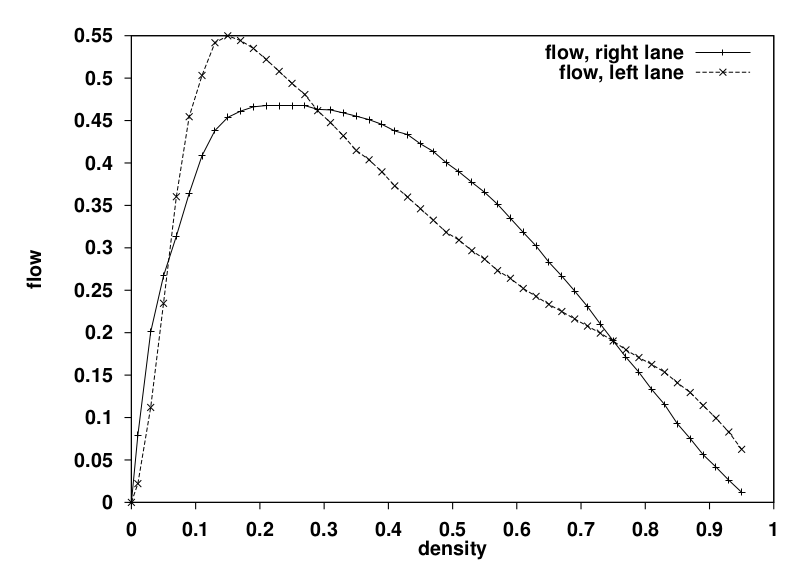
\includegraphics[width=0.75\textwidth]{verkehrsfluss}
 \caption[Verkehrsfluss als Funktion der durchschnittlichen Verkehrsdichte]{Verkehrsfluss auf den Fahrspuren als Funktion der durchschnittlichen Verkehrsdichte, aus \cite{multi-lane}}
 \label{figure:verkehrsfluss}
\end{figure}

Die Festlegung einer Wahrscheinlichkeit für das Zurückwechseln von der linken auf die rechte Fahrspur führte zu einer unterschiedlichen Spurwechselfrequenz, siehe \cref{figure:spurwechselfrequenz}.

\begin{figure}[hptb]
 \centering
 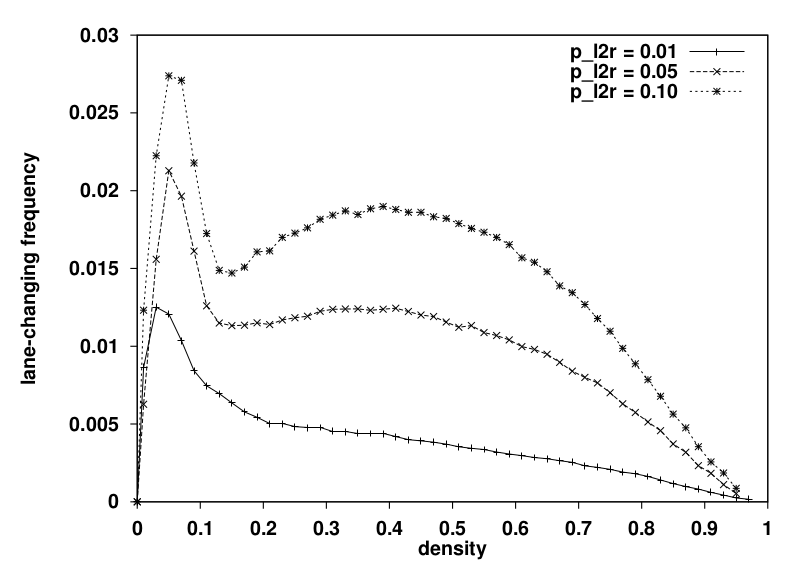
\includegraphics[width=0.75\textwidth]{spurwechselfrequenz}
 \caption[Spurwechselfrequenz als Funktion der Verkehrsdichte]{Spurwechselfrequenz als Funktion der Verkehrsdichte für verschiedene Spurwechselwahrscheinlichkeiten, aus \cite{multi-lane}}
 \label{figure:spurwechselfrequenz}
\end{figure}

In \cite{dat-ba} wurde für die Simulation der Spurwechsel eine "Social Forces"-Berechnung in Verbindung mit einer "Fitness Proportionate Selection"-Komponente erweitert. 
Durch gezielte Beachtung des umgebenden Verkehrs und dem Bewerten der zur Wahl stehenden Alternativen soll es möglich sein, das menschliche Verhalten besser als bisher abzubilden.\sa{Das hier ist eine Vermutung, also genau Deine Forschungsfrage das zu beweisen, kommt also ins nächste Kapitel} \\
"Social Forces" ist eine Simulationsmöglichkeit, die aus der Betrachtung von Menschenansammlungen kommt. 
Das Verhalten des Entscheiders Mensch, was auch im Straßenverkehr eine Rolle spielt, aber bisher in diesem Zusammenhang eher als eine Art "Black Box" betrachtet wurde, kann hiermit simuliert werden, um z.B. Evakuierungs- oder Panikszenarios zu veranschaulichen.\\
Der Hang zum Wechsel oder zur Beibehaltung der Spur wird hier nunmehr nicht nur durch eine fest vorgegebene Wahrscheinlichkeit simuliert, sondern durch eine individuell für jedes Fahrzeug zu jedem Zeitschritt berechnete "Kräfte", deren 'Entscheidung', durch entsprechende berechnete Wahrscheinlichkeiten getragen, mehr oder weniger häufig zur Ausführung kommen. 